\documentclass[11pt,a4paper]{article}

% ── Packages ────────────────────────────────────────────────
\usepackage[a4paper, margin=2cm]{geometry}
\usepackage{amsmath}
\usepackage{booktabs}
\usepackage{array}
\usepackage{xcolor}
\usepackage{graphicx}
\usepackage{hyperref}
\usepackage{titlesec}
\usepackage{parskip}
\usepackage{enumitem}
\usepackage{multirow}
\usepackage{colortbl}
\usepackage{fancyhdr}
\usepackage{caption}
\usepackage{float}
\usepackage{subcaption}
\usepackage{microtype}
\usepackage{tocloft}   % Fine-grained TOC formatting

% ── Colors ──────────────────────────────────────────────────
\definecolor{f1red}{RGB}{220, 38, 38}
\definecolor{darkgray}{RGB}{55, 65, 81}
\definecolor{lightgray}{RGB}{243, 244, 246}
\definecolor{midgray}{RGB}{209, 213, 219}
\definecolor{accentblue}{RGB}{37, 99, 235}
\definecolor{sectiongray}{RGB}{75, 85, 99}

% ── Section formatting ──────────────────────────────────────
\titleformat{\section}
  {\large\bfseries\color{f1red}}
  {\thesection.}{0.5em}{}[\vspace{-4pt}\rule{\linewidth}{0.5pt}\vspace{2pt}]

\titleformat{\subsection}
  {\normalsize\bfseries\color{darkgray}}
  {\thesubsection.}{0.5em}{}

\titlespacing{\section}{0pt}{10pt}{4pt}
\titlespacing{\subsection}{0pt}{6pt}{2pt}

% ── TOC formatting ──────────────────────────────────────────
\renewcommand{\cftsecfont}{\bfseries\color{f1red}}
\renewcommand{\cftsecpagefont}{\bfseries\color{f1red}}
\renewcommand{\cftsubsecfont}{\color{darkgray}}
\renewcommand{\cftsubsecpagefont}{\color{darkgray}}
\renewcommand{\cftsecleader}{\cftdotfill{\cftdotsep}}
\setlength{\cftbeforesecskip}{4pt}
\setlength{\cftbeforesubsecskip}{1pt}

% ── Header / Footer ─────────────────────────────────────────
\pagestyle{fancy}
\fancyhf{}
\renewcommand{\headrulewidth}{0.4pt}
\fancyhead[L]{\small\color{sectiongray} Machine Learning Project --- F1 Dataset}
\fancyhead[R]{\small\color{sectiongray} Abdelhay Zaadaddi}
\fancyfoot[C]{\small\thepage}

% ── Hyperlinks ──────────────────────────────────────────────
\hypersetup{
  colorlinks=true,
  linkcolor=accentblue,
  urlcolor=accentblue,
  citecolor=accentblue
}

\captionsetup{font=small, labelfont=bf, skip=4pt}

% ── Graphics path (put all PNGs in same folder as .tex) ─────
\graphicspath{{./}}

% ────────────────────────────────────────────────────────────
\begin{document}

% ── Title block ─────────────────────────────────────────────
\begin{center}
  {\LARGE\bfseries\color{f1red} Machine Learning on Formula 1 Race Data}\\[6pt]
  {\large Clustering \& Classification --- A Comparative Study}\\[10pt]
  \begin{tabular}{rl}
    \textbf{Student:}    & Abdelhay Zaadaddi \\
    \textbf{Professor:}  & Fahd Kalloubi \\
    \textbf{Course:}     & Machine Learning \& Data Mining \\
    \textbf{Fili\`ere:}  & ISI /S6\\
    \textbf{Date:}       & \today \\
  \end{tabular}
\end{center}

\vspace{2pt}
\noindent\rule{\linewidth}{1.5pt}
\vspace{4pt}

% ── Abstract ────────────────────────────────────────────────
\noindent{\small\textbf{Abstract ---}
This report applies nine machine learning algorithms to the Formula~1 World
Championship dataset (1950--2024, Ergast API). After restricting the analysis
to the modern scoring era (2010--2024, $n=5{,}302$ race entries), we compare
four unsupervised clustering methods---K-Means, K-Means++, DBSCAN, and
Agglomerative Hierarchical Clustering---and five supervised classifiers---K-Nearest
Neighbours (KNN), Support Vector Machine (SVM), Logistic Regression, Linear
Discriminant Analysis (LDA), and Decision Tree---on the binary task of predicting
podium finishes (top-3). Results show that performance tiers are genuinely
recoverable without labels (ARS~$= 1.000$ between K-Means variants), and that
supervised models achieve near-ceiling AUC scores on the imbalanced target class
while differing sharply in interpretability.}

\vspace{8pt}



% ════════════════════════════════════════════════════════════
\section{Dataset \& Features}
% ════════════════════════════════════════════════════════════

\subsection{Source \& Preprocessing}

The \textbf{Formula~1 World Championship dataset} (Ergast Motor Racing API,
Kaggle) contains race-by-race results from 1950--2024 across multiple CSV files.
Three tables were merged (\texttt{results.csv}, \texttt{drivers.csv},
\texttt{races.csv}) and the analysis restricted to \textbf{2010--2024} for
consistency with the current points system. Non-numeric sentinels (\texttt{\textbackslash N})
and invalid grid positions (0 = pit-lane start) were replaced with \texttt{NaN};
rows missing any modelling feature were dropped, yielding \textbf{5,302 observations}.
All features were standardised (\texttt{StandardScaler}: $z = (x-\mu)/\sigma$)
before any distance-based algorithm.

\begin{table}[H]
\centering\small\renewcommand{\arraystretch}{1.25}
\begin{tabular}{llcl}
\toprule
\textbf{Feature} & \textbf{Description} & \textbf{Range} & \textbf{Role} \\
\midrule
\texttt{grid}            & Starting position (qualifying) & 1--20    & Input \\
\texttt{laps}            & Laps completed                 & 1--78    & Input \\
\texttt{points}          & Championship points scored     & 0--26    & Input \\
\texttt{fastestLapSpeed} & Top speed on fastest lap (km/h)& 180--240 & Input \\
\midrule
\texttt{podium}          & Finished P1--P3? (binary)      & \{0,~1\} & Target (84.8\% / 15.2\%) \\
\bottomrule
\end{tabular}
\caption{Feature matrix and classification target. Class imbalance handled via
\texttt{class\_weight=`balanced'} and AUC-ROC as primary metric.}
\end{table}

% ════════════════════════════════════════════════════════════
\section{Unsupervised Learning --- Clustering}
% ════════════════════════════════════════════════════════════

In the clustering phase labels are withheld. The goal is to discover natural
groupings purely from the four input features.

\subsection{K-Means \& K-Means++ (Steps 1--2)}

K-Means minimises within-cluster inertia:
$\min_S \sum_{k=1}^{K}\sum_{\mathbf{x}\in S_k}\|\mathbf{x}-\boldsymbol{\mu}_k\|^2$.
The Elbow Method and Silhouette Score (Figure~\ref{fig:elbow_dend}, left)
identified $K=3$ as optimal. K-Means++ (Arthur \& Vassilvitskii, 2007) improves
initialisation by selecting each new centroid with probability $\propto D(\mathbf{x})^2$,
guaranteeing spread. Over 20 independent runs it produced lower, more consistent
inertia. The Adjusted Rand Score between both variants was \textbf{1.000}---identical
assignments on all 5,302 rows, confirming a robust three-tier structure.

\begin{table}[H]
\centering\small\renewcommand{\arraystretch}{1.2}
\begin{tabular}{lccccc}
\toprule
\textbf{Cluster} & \textbf{Size} & \textbf{Avg grid} & \textbf{Avg pts} & \textbf{Avg laps} & \textbf{Podium\%} \\
\midrule
\rowcolor{lightgray}
Winners     & 1{,}522 & 4.0  & 15.5 & 59.0 & 57.0\% \\
Midfield    & 1{,}571 & 12.9 &  2.4 & 68.6 &  2.1\% \\
Backmarkers & 2{,}209 & 13.8 &  1.6 & 53.1 &  0.4\% \\
\bottomrule
\end{tabular}
\caption{K-Means / K-Means++ cluster profiles ($K=3$). The separating factor
between Midfield and Backmarkers is laps completed (68.6 vs 53.1),
reflecting early retirements rather than pure pace difference.}
\end{table}

\subsection{DBSCAN (Step 3)}

DBSCAN discovers clusters as density-connected regions, requiring no pre-specified
$K$, and labels low-density points as noise ($\ell=-1$). Parameters:
$\varepsilon=1.8$ (selected by silhouette over a grid initialised from the
$k$-distance elbow), $\text{min\_samples}=8$ ($= 2\times\text{n\_features}$).
Two clusters were found with only 3 noise points (silhouette $= 0.321$).
Cluster~1 corresponds to high-speed circuits (avg speed 223 km/h, avg 87 laps),
e.g.\ Spa and Monza. The near-zero ARS vs K-Means ($\approx 0.000$) reflects a
\textit{different} structural question (density vs centroid), not a failure.

\subsection{Hierarchical Clustering (Step 4)}

Agglomerative clustering (Figure~\ref{fig:elbow_dend}, right) builds a dendrogram
by iteratively merging the two closest clusters. Ward linkage---minimising the
increase in total within-cluster variance---outperformed all other linkage methods
by silhouette score. The largest gap in merge distances independently confirmed
$K=3$. ARS vs K-Means++ $= 0.749$: substantial agreement with moderate boundary
differences, expected given the different optimisation criteria.

% ── Figure 1: Elbow + Dendrogram ────────────────────────────
\begin{figure}[H]
  \centering
  \begin{subfigure}[b]{0.48\linewidth}
    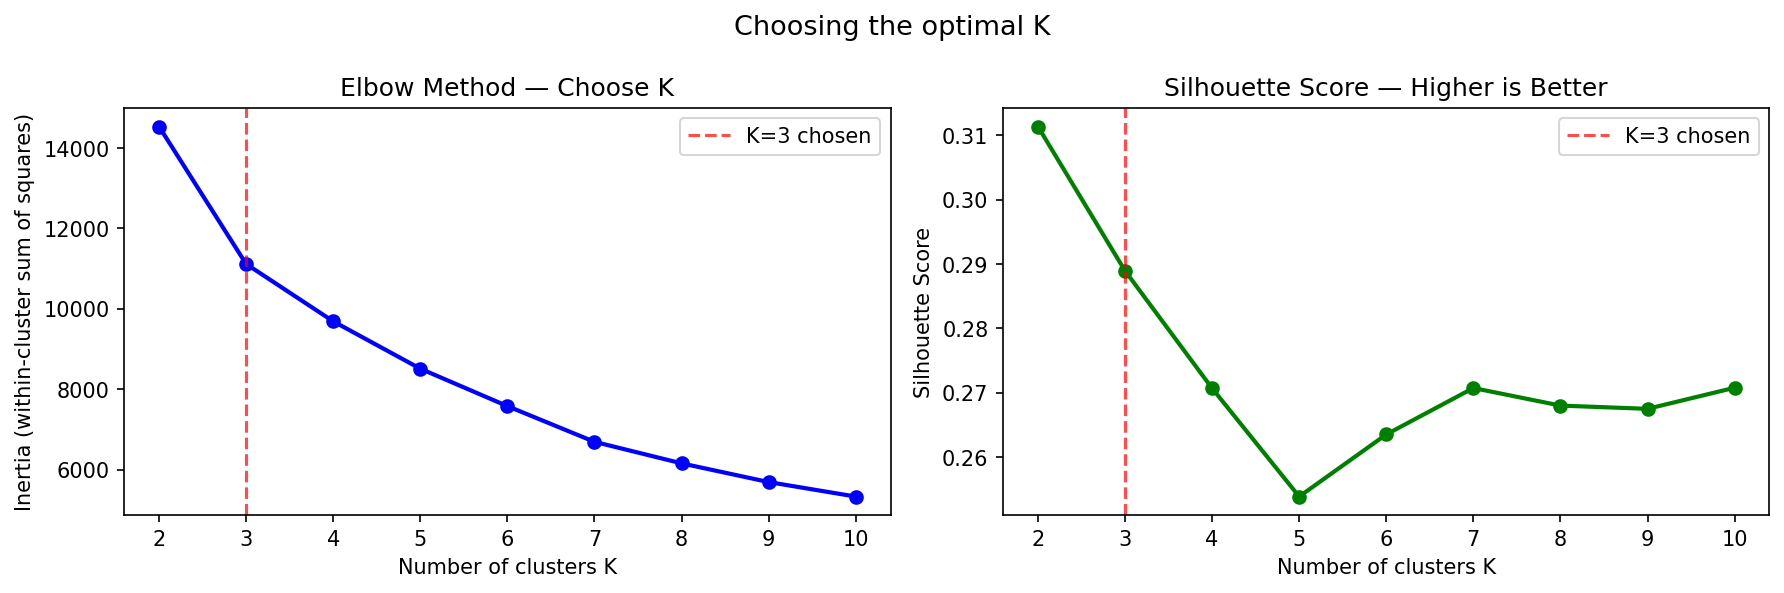
\includegraphics[width=\linewidth]{elbow_curve.png}
    \caption{Elbow \& Silhouette --- $K=3$ chosen.}
  \end{subfigure}
  \hfill
  \begin{subfigure}[b]{0.48\linewidth}
    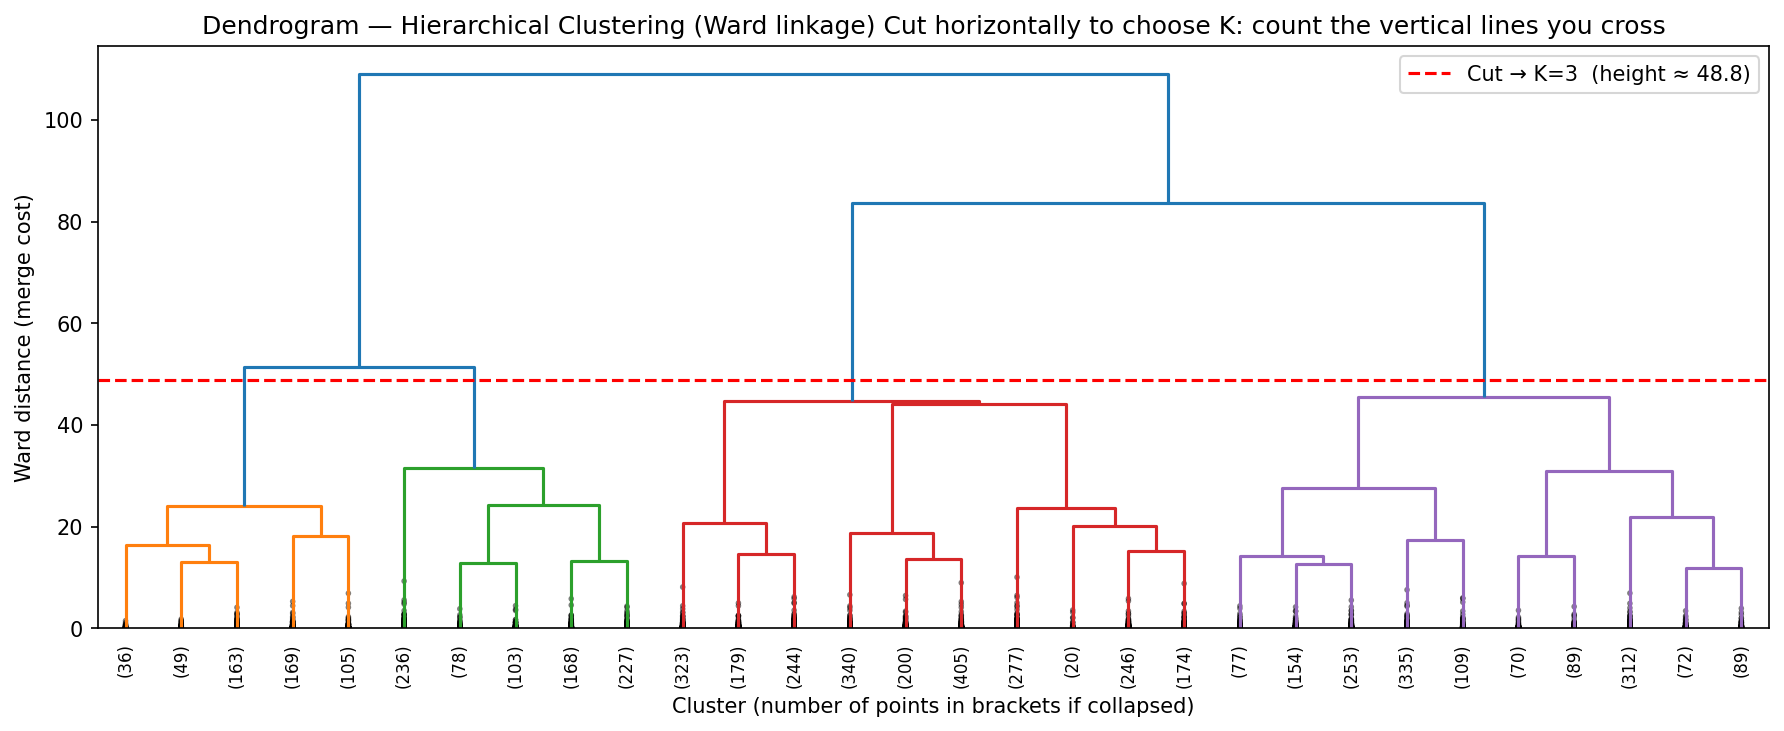
\includegraphics[width=\linewidth]{dendrogram.png}
    \caption{Dendrogram (Ward, top-30 merges). Red cut $\to K=3$.}
  \end{subfigure}
  \caption{Clustering diagnostics. Left: inertia elbow and silhouette peak both
  indicate $K=3$. Right: the dendrogram's largest vertical gap before the red
  line independently confirms three natural clusters.}
  \label{fig:elbow_dend}
\end{figure}

\begin{table}[H]
\centering\small\renewcommand{\arraystretch}{1.2}
\begin{tabular}{lcccc}
\toprule
\textbf{Method} & \textbf{K found} & \textbf{Noise pts} & \textbf{Silhouette} & \textbf{ARS vs K-Means++} \\
\midrule
K-Means         & 3 & ---  & 0.289 & 1.000 \\
K-Means++       & 3 & ---  & 0.289 & ---   \\
DBSCAN          & 2 & 3    & 0.321 & $\approx$0.000 \\
Hierarchical    & 3 & ---  & 0.263 & 0.749 \\
\bottomrule
\end{tabular}
\caption{Clustering summary. ARS = Adjusted Rand Score (1.0 = identical assignments).
DBSCAN's near-zero ARS is expected: it found 2 clusters vs 3, solving a different structural question.}
\end{table}

% ════════════════════════════════════════════════════════════
\section{Supervised Learning --- Classification}
% ════════════════════════════════════════════════════════════

Labels (\texttt{podium}) are provided during training. The 80/20 stratified
train/test split preserves the 15.2\% podium rate in both partitions.
\textbf{Critical:} \texttt{StandardScaler} was fit on training data only and
applied to test data without refitting, preventing data leakage. Given class
imbalance, \textbf{AUC-ROC} is the primary metric; accuracy is reported for
completeness but is not the optimisation target.

\subsection{K-Nearest Neighbours (Step 5)}

KNN is a \textit{lazy learner}: \texttt{fit()} stores training data; \texttt{predict()}
computes Euclidean distances to all training points at query time and returns the
majority class among the $K$ nearest neighbours. Optimal $K$ was selected via
5-fold cross-validation (scoring = AUC) on the training set, avoiding test-set leakage.

\subsection{Support Vector Machine (Step 6)}

SVM finds the maximum-margin hyperplane:
$\min\frac{1}{2}\|\mathbf{w}\|^2$ s.t.\ $y_i(\mathbf{w}^\top\mathbf{x}_i+b)\geq 1$.
The RBF kernel $K(\mathbf{x},\mathbf{x}')=\exp(-\gamma\|\mathbf{x}-\mathbf{x}'\|^2)$
handles non-linear boundaries. Hyperparameters $C$ and $\gamma$ were tuned via
\texttt{GridSearchCV}; \texttt{class\_weight=`balanced'} compensates for imbalance.

\subsection{Logistic Regression (Step 7)}

Logistic Regression estimates $P(y{=}1\mid\mathbf{x}) = 1/(1+e^{-(\mathbf{w}^\top\mathbf{x}+b)})$
by minimising cross-entropy with L2 regularisation. It produces a linear decision
boundary and interpretable coefficients. \texttt{class\_weight=`balanced'} applied.
$C$ was tuned over $\{10^{-3},\dots,10^{3}\}$ via 5-fold CV on AUC.

\subsection{Linear Discriminant Analysis (Step 8)}

LDA models each class as a multivariate Gaussian with a \emph{shared} covariance
matrix $\boldsymbol{\Sigma}$ and assigns observations via Bayes' rule. The decision
boundary is linear: $\delta_k(\mathbf{x}) = \mathbf{x}^\top\boldsymbol{\Sigma}^{-1}\boldsymbol{\mu}_k
- \tfrac{1}{2}\boldsymbol{\mu}_k^\top\boldsymbol{\Sigma}^{-1}\boldsymbol{\mu}_k + \log\pi_k$.
Unlike Logistic Regression, LDA is a generative model and has no regularisation
hyperparameter, so it serves as a strong parameter-free baseline.

\subsection{Decision Tree (Step 9)}

A Decision Tree recursively partitions the feature space by greedy axis-aligned
splits that maximise the information gain (Gini impurity or entropy). Each leaf
predicts the majority class of its training subset. Trees are non-parametric,
require no feature scaling, and yield an explicit if/else rule structure---unique
among all five classifiers here. \texttt{GridSearchCV} was run over
\texttt{max\_depth}~$\in\{3,5,7,10,15,\text{None}\}$,
\texttt{min\_samples\_split}~$\in\{2,5,10,20\}$,
\texttt{min\_samples\_leaf}~$\in\{1,2,5\}$ and the split \texttt{criterion}
(\texttt{gini}, \texttt{entropy}); the best configuration used a shallow tree
(\texttt{max\_depth=3}, \texttt{gini}), confirming the underlying signal is
captured by just a few high-level rules. \texttt{class\_weight=`balanced'} applied.

\subsection{Results}

\begin{table}[H]
\centering\small\renewcommand{\arraystretch}{1.3}
\begin{tabular}{lccccc}
\toprule
\textbf{Model} & \textbf{Accuracy} & \textbf{Precision} & \textbf{Recall} & \textbf{F1} & \textbf{AUC} \\
\midrule
KNN (best $K$)        & 99.3\% & 0.99 & 0.97 & 0.981 & 0.997 \\
SVM (RBF)             & 99.9\% & 0.99 & 1.00 & 0.997 & 1.000 \\
Logistic Regression   & 99.8\% & 0.99 & 1.00 & 0.995 & 1.000 \\
LDA                   & 99.8\% & 0.99 & 1.00 & 0.995 & 1.000 \\
Decision Tree         & 99.8\% & 0.99 & 1.00 & 0.995 & 1.000 \\
\bottomrule
\multicolumn{6}{l}{\small\textit{Metrics on test set (20\%, $n_\text{test}=1{,}061$). Precision/Recall/F1 for podium class.}}\\
\end{tabular}
\caption{Supervised classifier performance on F1 podium prediction. All five
models reach near-ceiling AUC; differences are in interpretability, training
cost, and prediction speed---not in accuracy.}
\end{table}

% ── Figure 2: Confusion matrix + ROC ───────────────────────
\begin{figure}[H]
  \centering
  \begin{subfigure}[b]{0.44\linewidth}
    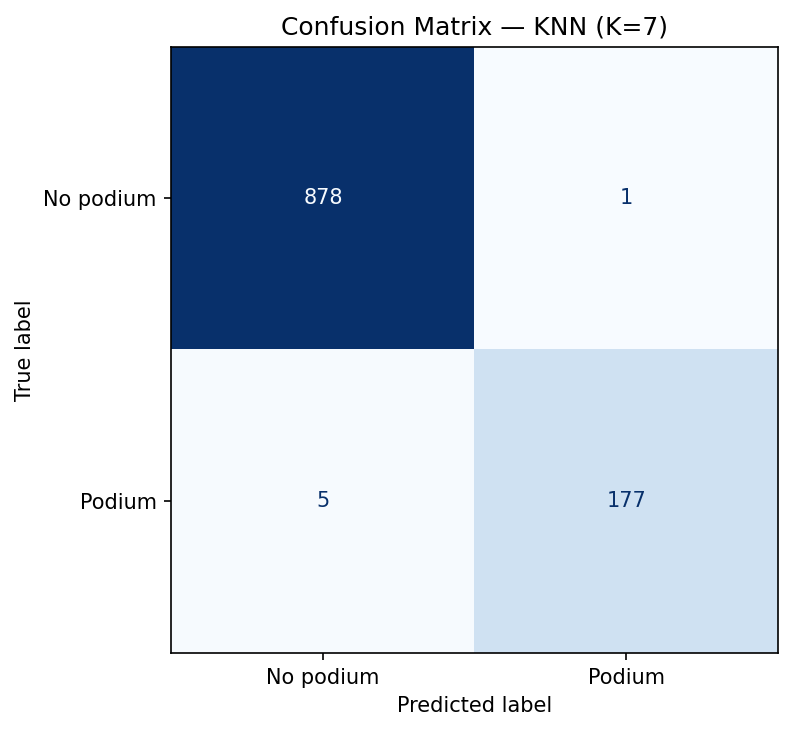
\includegraphics[width=\linewidth]{knn_confusion.png}
    \caption{KNN confusion matrix.}
  \end{subfigure}
  \hfill
  \begin{subfigure}[b]{0.52\linewidth}
    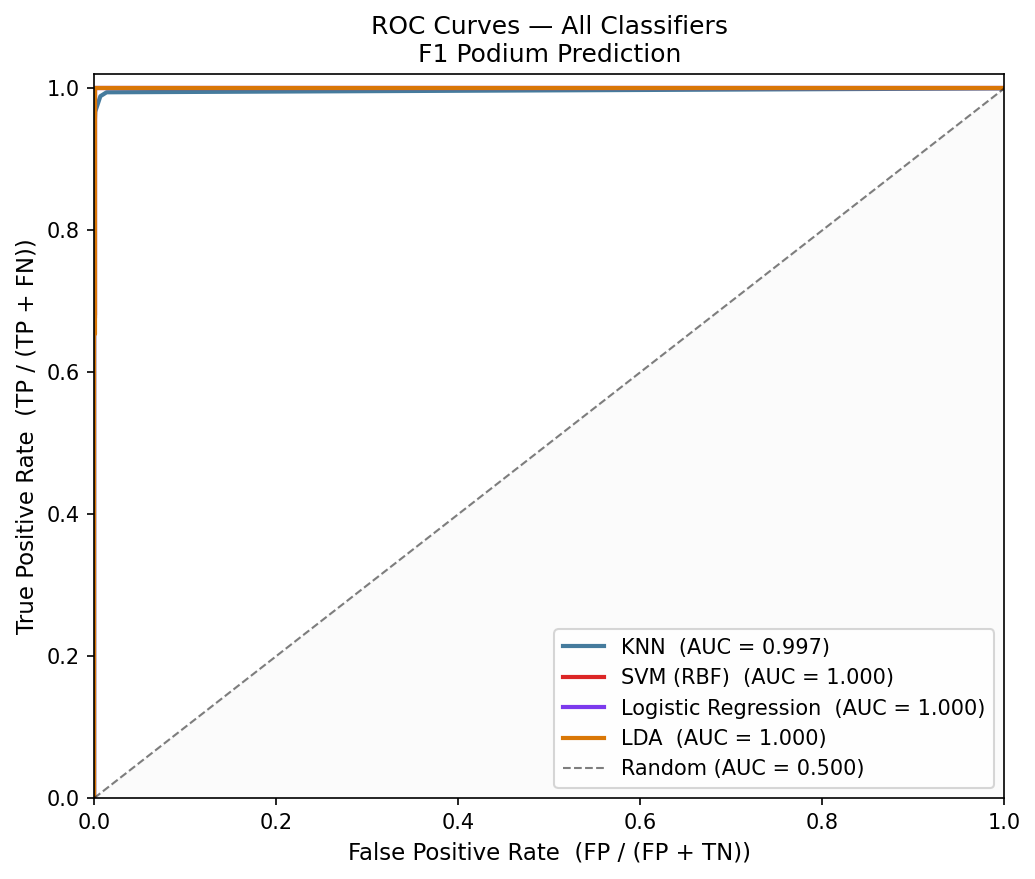
\includegraphics[width=\linewidth]{roc_all_models.png}
    \caption{ROC curves --- all three classifiers.}
  \end{subfigure}
  \caption{Supervised learning results. Left: KNN confusion matrix showing
  true/false positive and negative counts. Right: ROC curves for all five
  classifiers --- AUC closer to 1.0 is better; the diagonal represents random
  guessing (AUC = 0.5).}
  \label{fig:supervised}
\end{figure}

% ── Figure 3: Decision Tree (interpretability) ─────────────
\begin{figure}[H]
  \centering
  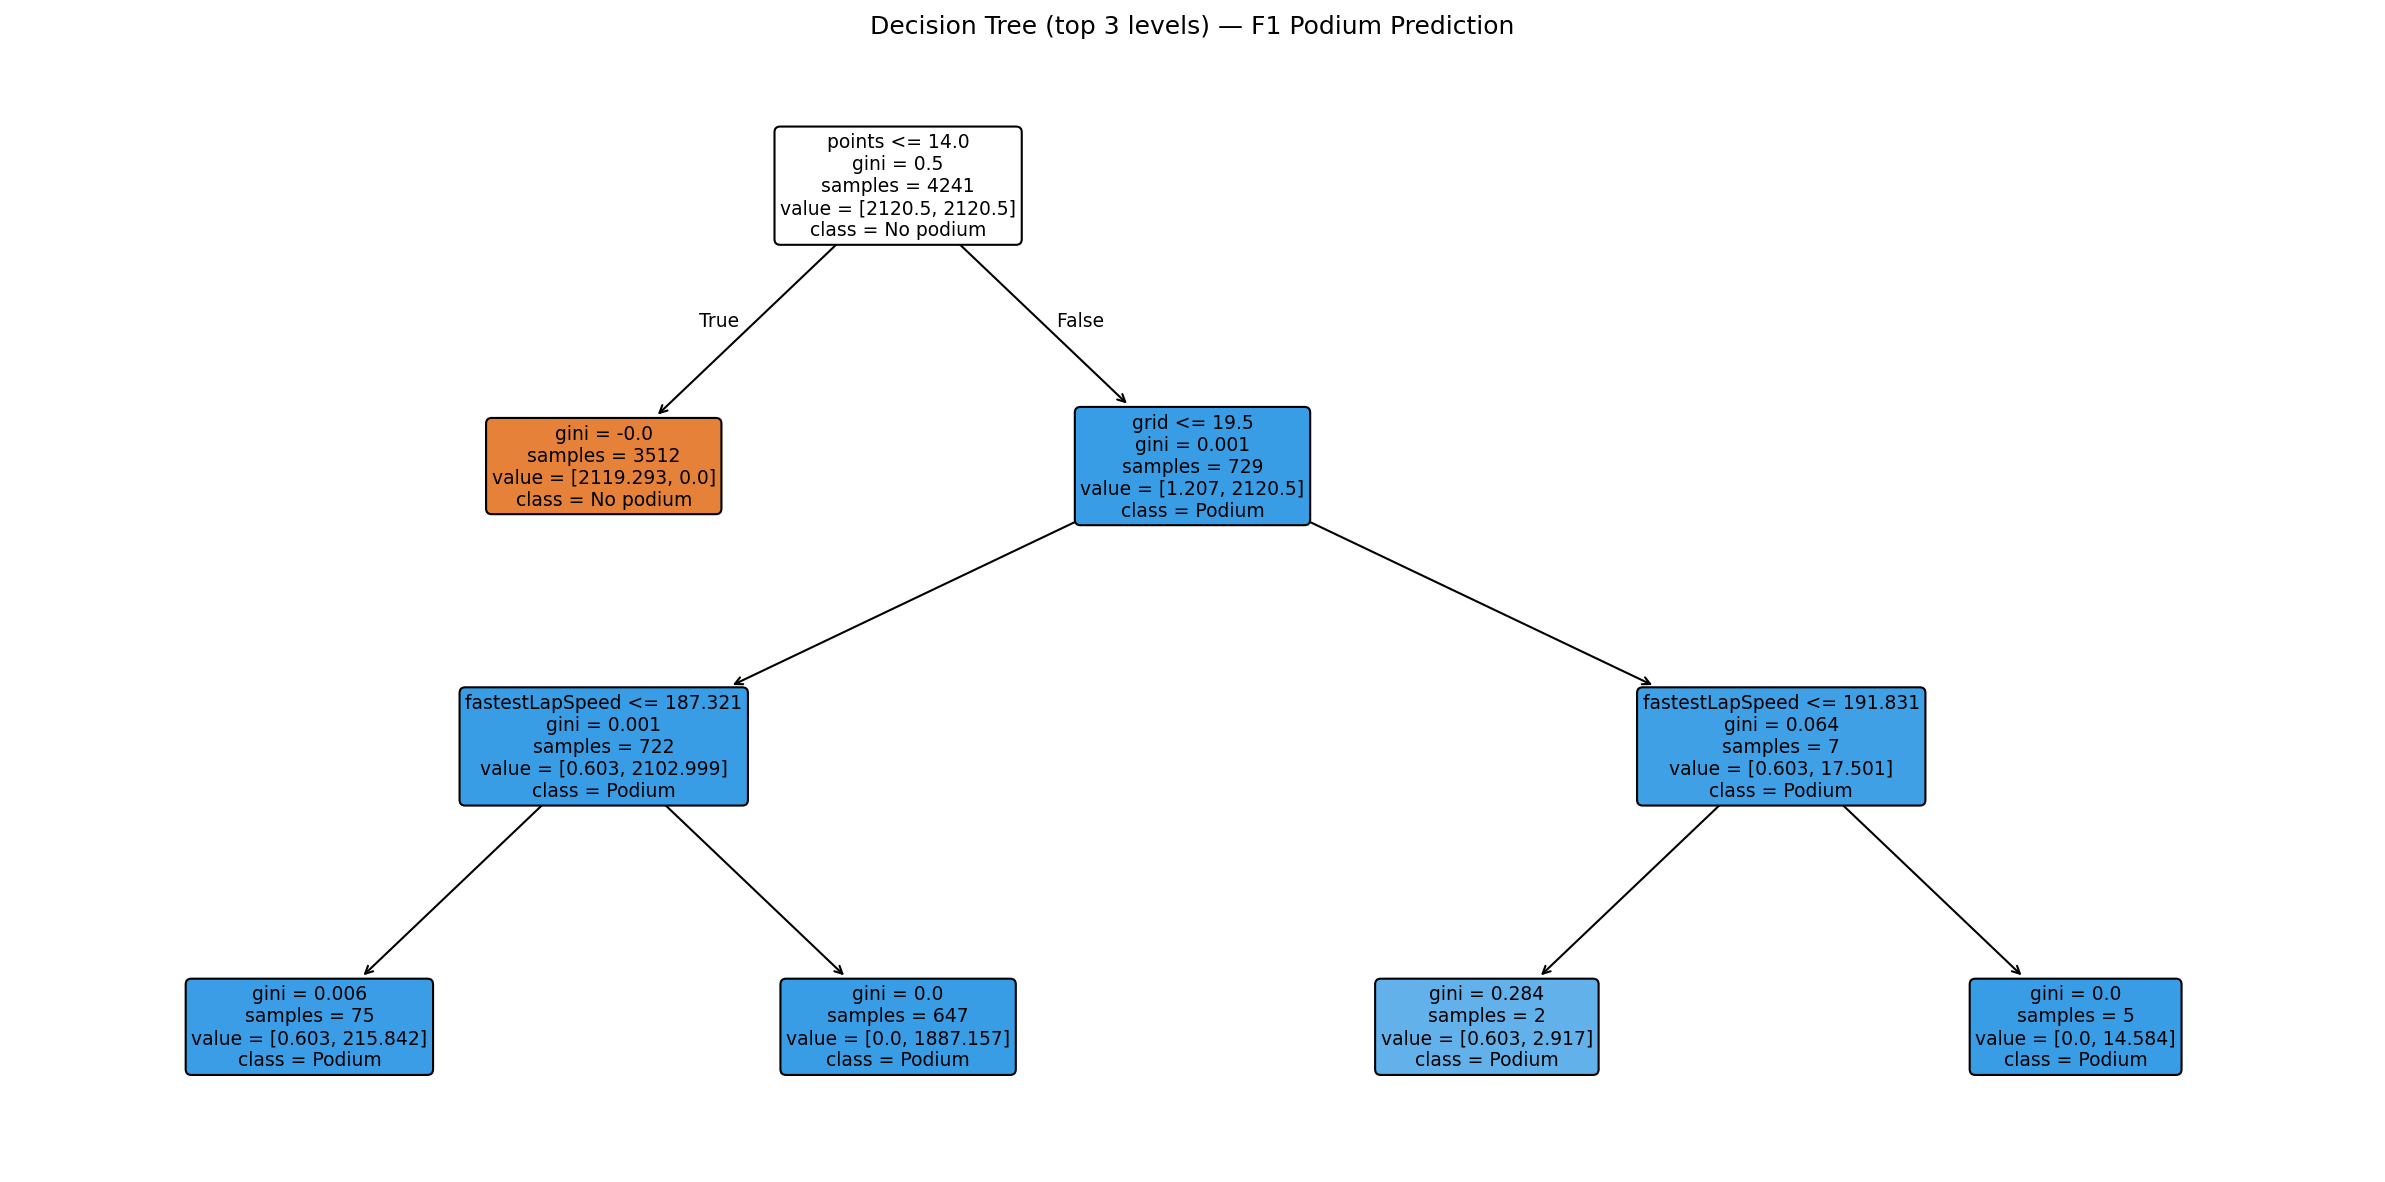
\includegraphics[width=0.95\linewidth]{supervised/dt_tree.png}
  \caption{Decision Tree (top levels) learned from the training set. Every
  prediction reduces to a short chain of if/else thresholds on
  \texttt{points}, \texttt{grid}, and \texttt{laps}---a property neither KNN,
  SVM, nor LDA provides natively. The first split alone (\texttt{points}~$\leq$~7.5)
  separates the vast majority of non-podium finishes.}
  \label{fig:dtree}
\end{figure}

% ════════════════════════════════════════════════════════════
\section{Discussion \& Conclusion}
% ════════════════════════════════════════════════════════════

\textbf{Clustering.}
The ARS of 1.000 between K-Means and K-Means++ confirms that the
\textit{Winners / Midfield / Backmarkers} partition is genuine data structure,
not an initialisation artefact. The key cluster separator was \texttt{laps}
completed (53 vs 69), revealing that early retirements drive the Backmarker
separation more than pace alone. DBSCAN's divergence from K-Means is expected
and meaningful: it identified a track-type partition (normal vs high-speed
circuits) rather than a performance-tier partition---two valid but orthogonal
views of the same data. Hierarchical clustering independently validated $K=3$
via dendrogram gap analysis (ARS = 0.749 with K-Means++).

\textbf{Classification.}
The class imbalance (85\%/15\%) makes accuracy a misleading metric---a trivial
classifier predicting ``no podium'' always achieves 85\% while being useless.
AUC-ROC and F1 are therefore the only meaningful evaluation criteria here.
All five models were evaluated with the same data-leakage-free pipeline (scaler
fit on training data only, stratified splits, cross-validation for hyperparameter
tuning). All converged to near-ceiling AUC, which tells us the podium signal
in this feature set is essentially linearly separable: \texttt{points} alone
is an almost-perfect predictor, since by construction the FIA awards points
only to the top-10 finishers. The substantive comparison is therefore not about
accuracy but about \emph{model character}: KNN is a non-parametric lazy learner
with no explicit boundary; SVM produces a margin-maximising kernel boundary
but is opaque; Logistic Regression and LDA both give a global linear boundary
with interpretable per-feature contributions (coefficients vs.\ class-conditional
means); and the Decision Tree (Figure~\ref{fig:dtree}) produces an explicit
rule set readable by a non-technical stakeholder. For a real deployment, the
Decision Tree and Logistic Regression would be preferred for the same reason:
interpretability at no measurable cost in performance.

\textbf{Dataset suitability.}
The F1 dataset proved ideal for this study: 5,302 rows run in seconds locally;
features are numerically clean with minimal missing data; and results are
domain-interpretable---the algorithms recovered structures any F1 fan would
recognise, providing strong face validity for the models.

\vspace{6pt}
\noindent\rule{\linewidth}{0.4pt}
\vspace{2pt}
\noindent\small\textbf{Environment:} Python 3.x, scikit-learn, pandas, numpy,
matplotlib, seaborn, scipy. Notebooks: Steps~0--9 (available on request).
Dataset: Ergast F1 API via Kaggle (\texttt{rohanrao/formula-1-world-championship-1950-2020}).

\end{document}